%\documentstyle[epsf,twocolumn]{jarticle}       %LaTeX2e仕様
%\documentclass[twocolumn]{jarticle}     %pLaTeX2e仕様(platex.exeの場合)
\documentclass[onecolumn]{ujarticle}     %pLaTeX2e仕様(uplatex.exeの場合)
%%%%%%%%%%%%%%%%%%%%%%%%%%%%%%%%%%%%%%%%%%%%%%%%%%%%%%%%%%%%%%
%%
%%  基本バージョン
%%
%%%%%%%%%%%%%%%%%%%%%%%%%%%%%%%%%%%%%%%%%%%%%%%%%%%%%%%%%%%%%%%%
\setlength{\topmargin}{-45pt}
%\setlength{\oddsidemargin}{0cm} 
\setlength{\oddsidemargin}{-7.5mm}
%\setlength{\evensidemargin}{0cm} 
\setlength{\textheight}{24.1cm}
%setlength{\textheight}{25cm} 
\setlength{\textwidth}{17.4cm}
%\setlength{\textwidth}{172mm} 
\setlength{\columnsep}{11mm}

%\kanjiskip=.07zw plus.5pt minus.5pt


% 【節が変わるごとに (1.1)(1.2) … (2.1)(2.2) と数式番号をつけるとき】
%\makeatletter
%\renewcommand{\theequation}{%
%\thesection.\arabic{equation}} %\@addtoreset{equation}{section}
%\makeatother

%\renewcommand{\arraystretch}{0.95} 行間の設定
%%%%%%%%%%%%%%%%%%%%%%%%%%%%%%%%%%%%%%%%%%%%%%%%%%%%%%%%
%\usepackage{graphicx}   %pLaTeX2e仕様(\documentstyle ->\documentclass)
\usepackage[dvipdfmx]{graphicx}
\usepackage{subcaption}
\usepackage{multirow}
%%%%%%%%%%%%%%%%%%%%%%%%%%%%%%%%%%%%%%%%%%%%%%%%%%%%%%%%
\begin{document}
	
	%bibtex用の設定
	%\bibliographystyle{ujarticle} 
	
	\noindent
	
	\hspace{1em}
	2019 年 6 月 21 日
	ゼミ資料
	\hfill
	M1 寺内 光
	
	\vspace{2mm}
	
	\hrule
	
	\begin{center}
		{\Large \bf 進捗報告}
	\end{center}
	
	
	\hrule
	\vspace{3mm}
	
	% ‚ここから 文章 Start!
	\section{パーツ抽出のためのモデル作成に向けて}
	ひとまず 1 番最初に思いつきそうなモデルを作成.図 \ref{fig:model} にモデル構造を示す.今まで使ってきた CAE モデルを 2 つ分岐させるようなモデル構造を定義した.
	入力画像としてオリジナル画像を入れ,ターゲットとして目抜き画像と目のみ画像を設定し,それぞれに関して binary cross entropy を最小化する学習を行う.問題点としては,MaxPooling 層を挟むことによって復元される画像がぼやけてしまうことが挙げられる.
	そこで MaxPooling 層を除いて学習させたが,出力の 1 つがオリジナル画像とほぼ同一になる学習をしてしまうことがわかった.図 \ref{fig:input_and_output} に入力画像と出力画像を示す.
	
	\section{Semantic Segmentation}
	やりたいことは Semantic Segmentation とほとんど同じ(ピクセルが目に属するものとそれ以外を取ってくればよい).
	4 コマ漫画ストーリーデータセットを使えば Semantic Segmentation を行うためのアノテーションとしては十分だと思われる.
	Semantic Segmentation のためのモデルには Fully Convolutional Networks for Semantic Segmentation \cite{DBLP:journals/corr/LongSD14}, SegNet \cite{badrinarayanan2015segnet2} や U-Net \cite{DBLP:journals/corr/RonnebergerFB15} があるらしい.最新の手法は Google の DeepLab-v3 \cite{DBLP:journals/corr/abs-1802-02611}.
	\begin{figure}[h]
		\begin{center}
			\vspace{-10mm}
			\hspace*{30mm}
			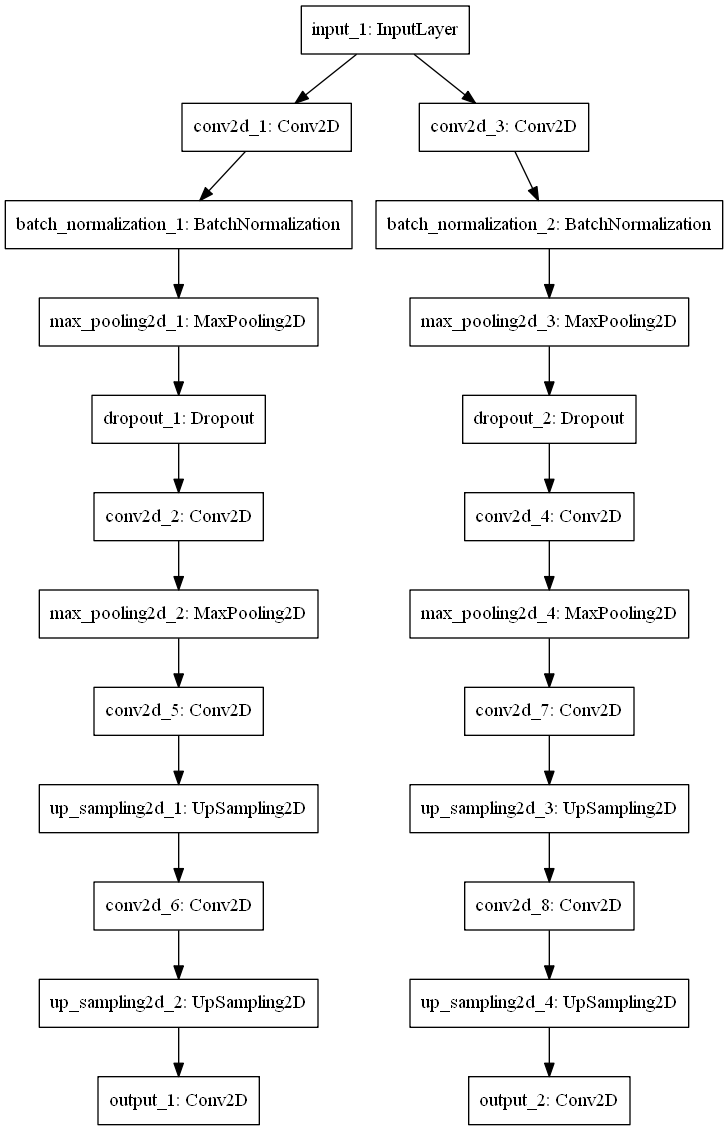
\includegraphics[width=0.9\columnwidth]{model_structure.png}
			\caption{パーツ抽出のためのモデル定義}
			\label{fig:model}
		\end{center}
	\end{figure}

	\begin{figure}[h]
		\vspace{-4mm}
		\centering
		\begin{subfigure}{0.49\columnwidth}
			\centering
			
\includegraphics[width=1.2\columnwidth]{original.png}
			\caption{オリジナル画像}
			\label{fig:original}
		\end{subfigure}
		\\
		\begin{subfigure}{0.49\columnwidth}
			\centering
			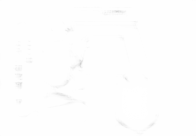
\includegraphics[width=1.2\columnwidth]{eyes_only_10.png}
			\caption{出力 1( ターゲット:目のみ画像 )}
			\label{fig:only_eye}
		\end{subfigure}
		\begin{subfigure}{0.49\columnwidth}
			\centering
			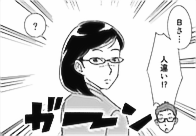
\includegraphics[width=1.2\columnwidth]{rem_eye_10.png}
			\caption{出力 2( ターゲット:目抜き画像 )}
			\label{fig:rem_eye}
		\end{subfigure}
		\caption{オリジナル画像とその出力}
		\label{fig:input_and_output}
	\end{figure}
	
	\section{Data Augmentation}
	現在,画像オーギュメンテーションの手法については 3 種類の方法を考えている.
	\begin{enumerate}
		\item 回転やスライド等のオーギュメンテーション (keras の ImageDataGenerator を使えばすぐできる)
		\item レイヤ抜きによるオーギュメンテーション
		\item 上記の両方を用いる
	\end{enumerate}

	\section{来週以降のタスク}
	\begin{enumerate}
		\item FCN, SegNet, U-Net の論文を読む
		\item 教師ラベル作成のためのジェネレータ定義(けっこう大変そう)
	\end{enumerate}
	
	% 参考文献リスト
	\bibliographystyle{unsrt}
	\bibliography{2019_06_21_terauchi}
\end{document}